\chapter{State of the art}
	
	The pick and place task that is intended to be performed in this thesis is really useful for a lot of applications into the industrial world because it would bring a lot of flexibility for these processes. A example of this applications could be an assembly line, where robotic arms could be picking all the different pieces to assemble in the product using always the same algorithm.
	
	Big companies are developing a lot of Artificial intelligence use cases in the industry, and they try to contribute to the AI community by publishing scientific articles on how they managed to use AI for their specific tasks. Unfortunately, although some companies have already developed their own solutions for our specific pick and place task, none of them have published a scientific article on the subject, making it difficult to study the way they have achieved it.
	
	One of the companies that has already developed a pick and place task is the Japanese automation company Fanuc, which has developed an AI-based solution together with Preferred Networks. As commented before, they have not published any scientific article about the topic but we can see the system working in a video they have posted on YouTube \cite{preferred_networks_inc_bin-picking_2015}. That means that we have to gather all the possible information from the video, where we could find that they have not used a Reinforcement Learning algorithm but just a Deep Neural Network (DNN) with image recognition. 
	
	To train the net, they have collected "success" or "fail" labelled images by making pick actions in random places of the box. Once they gathered a big enough dataset of images, they have trained a Deep Neural Network as the one we see in \autoref{fig:fanucdnn}, where we can also see that the Neural Net has been trained to predict whether the robot is going to success in a pick action in a specific place or not. Using that net, they can make a heat map of the whole box, predicting the points of maximum probabilities of succeed. As usually, they noticed that the bigger the image dataset, the higher the success ratio. In eight hours, they reach 90\% of success, which they say is bigger than the human success ratio.
	
	\begin{figure}
		\centering
		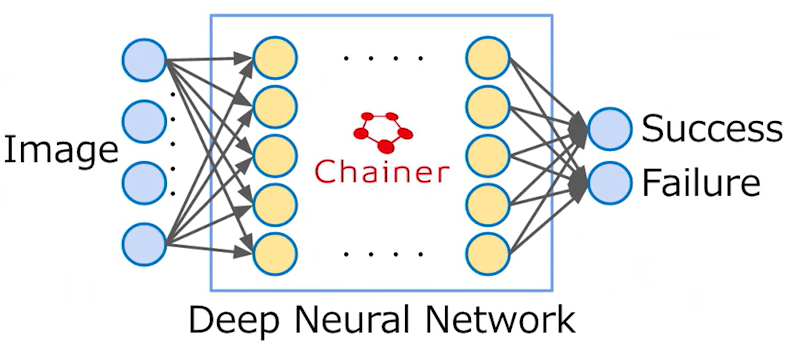
\includegraphics[width=0.85\linewidth]{Images/FANUC_DNN.png}
		\caption[Fanuc DNN]{Deep Neural Network of Fanuc solution (taken from the video)}
		\label{fig:fanucdnn}
	\end{figure}
	
	\subsection{Reinforcement Learning}
	
		The idea of the project is to keep using image recognition techniques but, in our case, applied to a \textbf{Reinforcement Learning} Algorithm which is an area of machine learning inspired by psychology behavioural. Its goal is to determine what actions a software agent should choose in a given environment in order to maximize some notion of "reward" or accumulated prize. 
		
		Explained easily, RL is used to make an \textbf{agent} (the robot) learn how to interact with a \textbf{environment} in order to perform a task. To achieve this, Markov Decision Process (MDP) which provides a mathematical framework for modeling decision making in situations where outcomes are partly random and partly under the control of a decision maker.
		
		\subsubsection{Markov Decision Process (MD)}
			In MDP, the environment is what we are actually trying to simulate with the MDP. The agent will interact with it to learn how to perform the task, so these are the attributes of the environment:
			\begin{itemize}
				\item[\textendash]\textbf{Agent:} The agent is the most important piece of the algorithm because it represents the objects that we want to become smarter.
				\item[\textendash]\textbf{Actions (A):} The agent can interact with the environment by performing a set of actions which is normally finite.
				\item[\textendash]\textbf{States (S): } Each time the agent performs an action, it moves to a new state. States are basically the set of information that differentiates the situation of the agent before and after performing an action. States can be transitional or terminal, when the agent meets the objective or when it gets to a forbidden position.
				\item[\textendash]\textbf{Rewards (R):} Each time an action is performed, the agent receives a reward. This reward can be positive, negative or null depending on the impact of the action to achieve the objective.
				\item[\textendash]\textbf{Policy ($\pi$):} The policy is used to define the optimal action for each step. It gives a punctuation for all of the actions in the current step as shown in the following formula. The agent takes the action with highest punctuation.
				\begin{gather*}
					\pi(a|s)=P_r\{A_t=a|S_t=s\}
				\end{gather*}
			
			\end{itemize}
			
			The MDP is divided in discrete timesteps (t), where each timestep does not have to last the same time as the previous step. Each timestep, the agent uses the policy $\pi$ to decide the next action. 
			
			Once the action is taken:
			\begin{itemize}
				\item[\textendash]The environment transits to th next state: \textbf{ \boldmath$S_t = S_{t+1}$}.
				\item[\textendash] Environment produces a new reward, which can be represented with the following formula: \boldmath
				\begin{gather*}
					P(s', r, s, a) = P_{r}\{S_{t+1}=s', R_{t+1}=r, S_{t}=s, A_{t}=a\}
				\end{gather*}
			\end{itemize}
			
			Agent's performance is calculated in terms of its future accumulated rewards known as return. This is called \textbf{expected return} an is calculated as  shown in the formula below, where $\gamma$ is the discount factor, and is used to give a bigger value to the closest steps.
			
			\begin{gather*}
				G_t = \sum_{k=t} \gamma ^{k-t} \cdot R_{k+1} \:\: \forall \:\: \gamma \in [0, 1]
			\end{gather*}
		
		
		\subsubsection{Q-Learning}
			
			Now that we know all these concepts, we have to learn what Reinforcement Learning Algorithms do to learn. Basically, \textbf{the goal of the agent is to find a policy that maximizes the expected return }. This can be done using different strategies as:
			\begin{itemize}
				\item[\textendash]\textbf{Q-Learning:} Estimating action values using Q Tables or other methods
				\item[\textendash]\textbf{TRPO:} Parametrizing the policy and optimizing its parameters
			\end{itemize}
			
			Basic Q-Learning is based on the assumption that both actions and states are limited and that the same action in the same state always drives to the same new state. Having this in mind, Q-learning algorithms build two matrices of shape \textbf{length(actions) x length(states)} as shown in the \autoref{fig:q-matrix}.
			
			\begin{figure}[h]
				\centering
				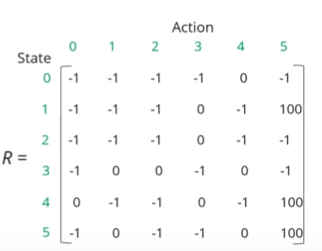
\includegraphics[width=0.7\linewidth]{Images/Q-Matrix}
				\caption[Q-Matrix]{Reward and Q Matrix shape in Basic Reinforcement Learning}
				\label{fig:q-matrix}
			\end{figure}
			
			In these two matrices, Q-Learning algorithm stores in the R matrix the reward for the pair of action-state while in the Q matrix they store cumulated reward for this same pair. The Q matrix is the one used to decide which action to perform in each state and R matrix the one used to calculate the reward of each action. 
			
			However, for the aim of this project, the states of the agent can be different in each timestep. The state would actually be partially formed by images, so the number of states can be infinite. We need a more complex version of Reinforcement Learning.
			
	\subsection{Deep Reinforcement Learning}
		
		The approach of mixing both image recognition and RL is called Deep Q Learning (DQN) or Double Deep Q Learning (DDQN) depending on the implementation and uses Neural Networks in two different stages of the algorithm. Firstly, a Convolutional Neural Network (CNN) is used to extract image features, and then, a Deep Neural Network (DNN) is used to calculate the q value of each independent action and select the next one using these values.
		
		DQL was proposed in 2012, and, since then, it has been used for a lot of different purposes. For example, Guillaume Lample and Devendra Singh Chaplot demonstrated back in 2017 that a RL agent could play FPS Games using as inputs just game scores and pixels from the screen \cite{lample_playing_2018}. Another really interesting example is this robot \cite{zhu_target-driven_2017}, which is capable of moving around a house looking for an objective and avoiding obstacles using DDQL.
		
		A good resource to understand how Reinforcement Learning really works is Deeplizard's tutorial \cite{noauthor_reinforcement_nodate}. In this tutorial they explain different versions of the algorithm and how to implement them in python to solve different OpenAI gym environments \cite{openai_gym_nodate}. 
		
		Deep Reinforcement Learning is though an union between RL and image recognition, but let's see how it actually works. The main idea is to replace the Q-table that we saw before for a Dense Neural Network that uses as input another Neural Network, a Convolutional Neural Network (CNN). The full algorithm would have as many outputs as allowed actions. Therefore, simplifying, these outputs re equivalent to the q-values saw before and so we will call them. To see it graphically, when the agent wanted to take an action, he  would pass the state image through the Neural network represented in \autoref{fig:deepqnetwork} and would take the action with higher q-value.
		
		\begin{figure}[h]
			\centering
			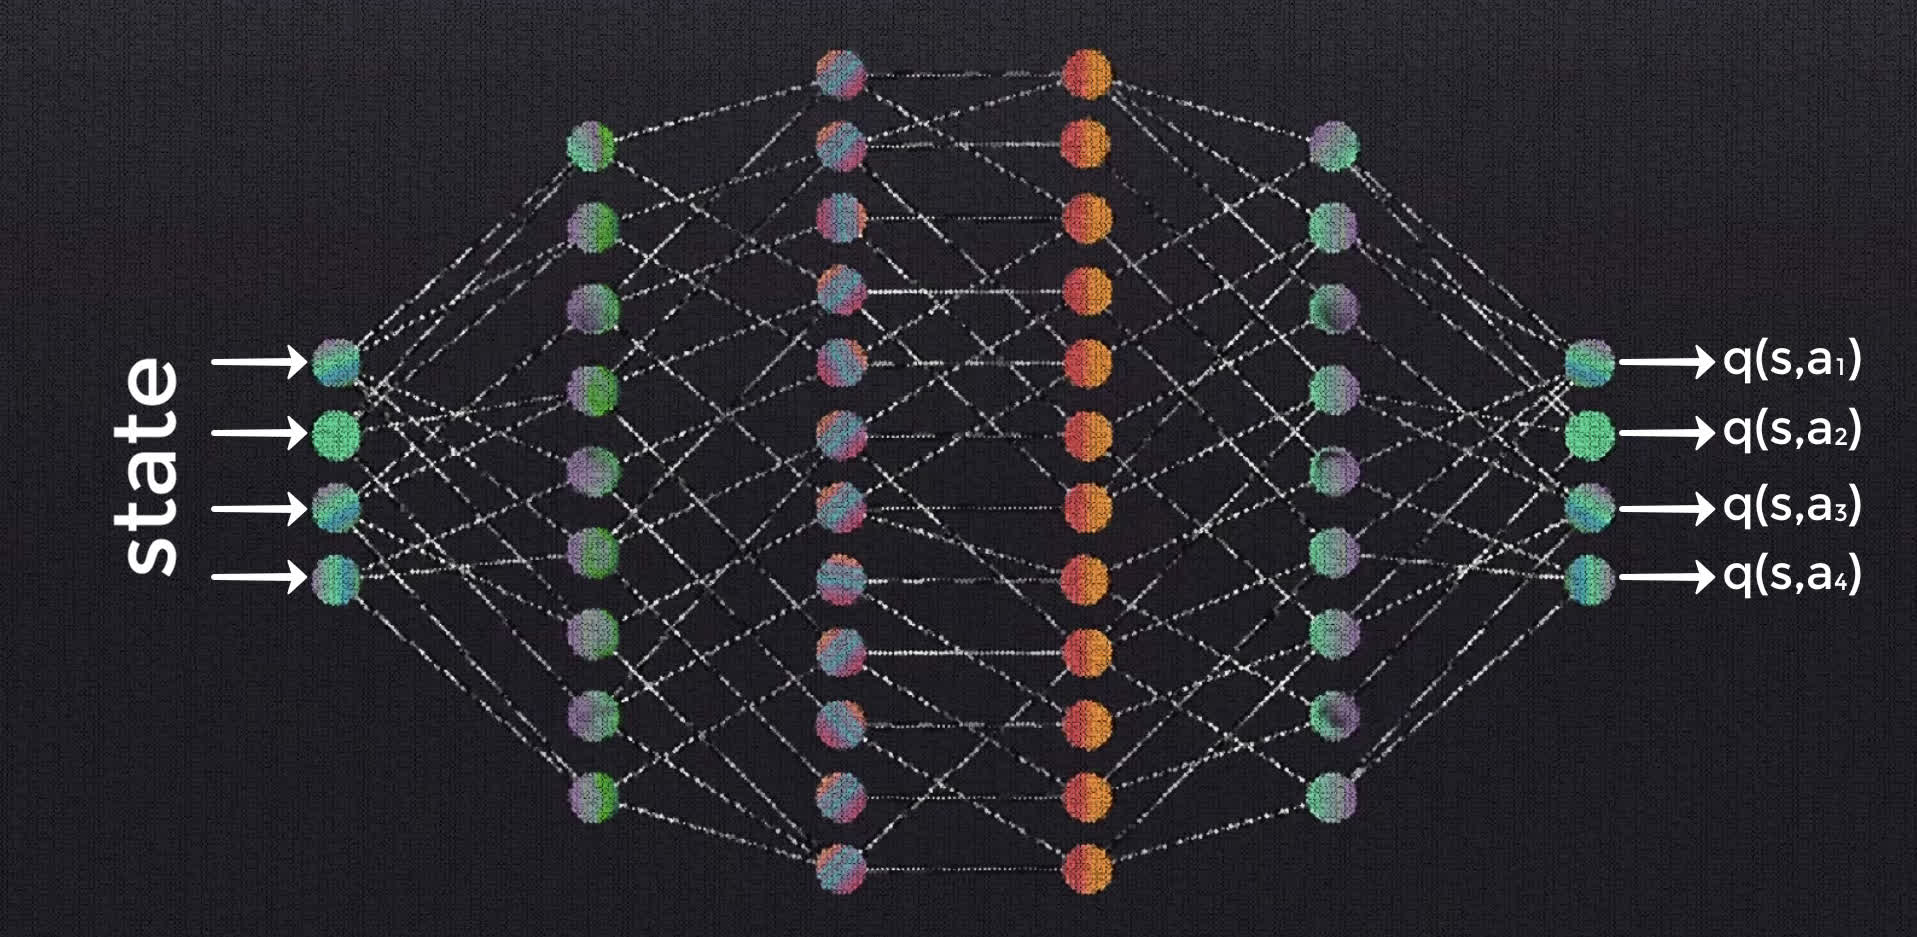
\includegraphics[width=0.7\linewidth]{Images/DeepQ-Network.jpg}
			\caption[Deep Q Learning]{Deep Q Learning Representation with 4 outputs}
			\label{fig:deepqnetwork}
		\end{figure}
		
		When I said "simplifying" in the previous paragraph, I meant "simplifying a lot" in the next paragraphs I will explain all the intermediate steps in the algorithm and why they are important:
		
		\begin{itemize}
			\item[\textendash]Episodes and Steps
			\item[\textendash]Exploration vs Exploitation trade-off
			\item[\textendash]Replay Memory
			\item[\textendash]Bellman's Equation
			\item[\textendash]Target and Policy Networks
		\end{itemize}
	
		\subsubsection{Episodes and Steps}
			RL training is divided in Episodes. One Episode is the sequence of actions needed to reach a terminal State. Each time the agent reaches a terminal state, an episode is ended, and a new one is started.
			
			On the other hand, steps represents every time that a new action is taken, so the number of steps taken by the agent during training is infinite. Later on, we will use as metric of performance the number of steps per episode, as they must decrease during the training.
		
		\subsubsection{Exploration vs Exploitation trade-off}
			In Reinforcement Learning there are two important concepts that are \textbf{Explore} and \textbf{Exploit}. To explore is basically gather new information about the environment and to exploit is to make the best decision with the information that we already have.
			
			In Deep Reinforcement Learning, the agent exploit the information gathered by using the pre-trained Neural Network to decide next action. On the other hand, the agent explore the environment by deciding next action randomly. We use exploration mainly in the beginning of the training because we want the agent to gather as much information of the environment as possible before starting training.
			
			When the agent uses exploitation, it is also gathering information about the environment. However, we could not let the agent explore this way because during the exploration phase we want all the actions to be performed with the same probability and neural network bias can cause some actions to be performed much more than others.
			
			So, how do we decide when the agent must explore or exploit? To decide it we can use multiple techniques, but the most common one is the Epsilon-Greedy Strategy. This strategy basically consist on setting a probability of exploring and keep decreasing it slowly during the training. It works this way:
			
			\textbf{\begin{enumerate}
				\item We set the initial exploring probability ($\epsilon$)
				\item We set the per-step epsilon decay, ($\epsilon\_decay$)
				\item For each step:
				\begin{enumerate}
					\item With probability $p = \epsilon$, the agent explores the environment (takes a random action). If not, it exploit the information by deciding the action using the NN.
					\item Whether the agent has explore or not, we decrease the probability of exploring the environment in the next step ($\epsilon = \epsilon - \epsilon\_decay$)
				\end{enumerate}
			\end{enumerate}}
			
			Using this strategy, the agent will rather explore or exploit the environment during the training. In the first steps the probability of a random action (exploring) will be much hihger than in the last steps of the algorithm. This probability will keep decreasing during the training, until it reaches the minimum exploring rate, which is normally set to 10%.
			
		
		\subsubsection{Replay Memory}
		
			Everytime that the agent performs an action, either by exploring or exploiting, the agent lives an experience. For the purpose of training the algorithm, we will store all these experiences.
			
			Experiences are formed by the initial state, the action taken, the state reached (final state) and the reward gotten and they are stored in the Replay Memory. Then, every time that an action is taken, the algorithm is trained following this steps:
			
			\begin{enumerate}
				\item Replay Memory checks if the number of experiences is higher than the batch size
				\item If there are enough experiences:
				\begin{enumerate}
					\item Replay Memory supplies a random set of experiences of size=batch\_size.
					\item With this set of experiences, the target network is trained.
				\end{enumerate}
			\end{enumerate}
			
			Optimizing Replay Memory can be a challenge, because, if we are using a Graphic Card in the training, we would be storing all the experiences in its memory. But, why do we need to store all the experiences? We could also be using the last N experiences to train the network and it would be a less memory-consumption demanding solution. 
			
The answer to this question is that Reinforcement Learning Networks converge really slowlly and variance between consecutive steps is really low. Using consecutive experiences to train the network would result though in a slower and biased learning. Besides, this way of working is better for learning real-world experience, where there are infinit different states, as the experience gainend in previous steps will be used multiple times later to train the network.


		\subsubsection{Bellman's Equation}
			\begin{gather*}
				q_*(s,a) = E[ R_{t+1} + \gamma max(q_*(s', a' )]
			\end{gather*}
			
			Suppose we have some arbitrary deep neural network that accepts states from a given environment as input. For each given state input, the network outputs estimated Q-values for each action that can be taken from that state. The objective of this network is to approximate the optimal Q-function, and remember that the optimal Q-function will satisfy the Bellman equation that we covered previously:

  
With this in mind, the loss from the network is calculated by comparing the outputted Q-values to the target Q-values from the right hand side of the Bellman equation, and as with any network, the objective here is to minimize this loss.


After the loss is calculated, the weights within the network are updated via SGD and backpropagation, again, just like with any other typical network. This process is done over and over again for each state in the environment until we sufficiently minimize the loss and get an approximate optimal Q-function.

So, take a second now to think about how we previously used the Bellman equation to compute and update Q-values in our Q-table in order to find the optimal Q-function. Now, with deep Q-learning, our network will make use of the Bellman equation to estimate the Q-values to find the optimal Q-function. So, we’re still solving the same general problem here, just with a different algorithm. Rather than making use of value iteration to solve the problem, we’re now using a deep neural network.
		
		\subsubsection{Target and Policy Networks}
		
		
		
		
		
		
		
	\subsection{Problems of Deep Reinforcement Learning in Real-world}
		
		Real-world problems introduces some challenges that we will have to manage. In march 2018, A. Rupam Mahmood, Dmytro Korenkevych, Brent J. Komer, and James Bergstra explained the problems they found while implementing a RL algorithm in a UR5 robotic arm \cite{mahmood_setting_2018}.
		
		Some of the problems they found were the following:
		
		\begin{itemize}
			\item[\textendash]Slow rate of data-collection, as movements in the real robot are slower than in a simulated environment. 
			\item[\textendash]Partial observability. Sensors cannot retrieve all the information about the environment.
			\item[\textendash]Noisy sensors will provide inaccurate information.
			\item[\textendash]Safety of the robot and its surroundings have to be taken in mind.			
			\item[\textendash]Fragility of robot components.
			\item[\textendash]Delay between an action is requested and the time it is actually performed can affect the training.
			\item[\textendash]Preparing the robot is a really difficult task:			
			\begin{itemize}
				\item[\textendash] Controlling the robot.
				\item[\textendash] Define all aspects of the environment.
				\item[\textendash] Difficulties for obtaining random and independent state when episode ends.
			\end{itemize}
		\end{itemize}
		
		Another problem that can be found in our project is that, as objects are randomly placed, the environment that the agent will have to face will be completely different each time. In fact, the robot can interact with the environment, as it can move the pieces trying to pick them, so we are facing a dynamic environment RL problem. A good example of a dynamic environment problem is the path planning of a self driven car, where each time the agent takes an action the environment will change and, furthermore, obstacles do not have to be static, but they can also move.
		
		%% TODO: Explicar en profundidad (En descripción de las tecnologías)
		There are multiple examples of articles on this topic, such as the one Xiaoyun Lei, Zhian Zhang, and Peifang Dong published in September 2018 using a DDQN approach to solve it \cite{lei_dynamic_2018}. However, there are other solutions as the one proposed by Marco A. Wiering \cite{wiering_reinforcement_2001}, where he introduces some prior knowledge to the model in order to facilitate the learning. His algorithm had problems generalizing the environment, so he introduced some prior information about the model together with a Model-based RL. This made the algorithm more capable to learn without loosing a lot of trainable capability.
		
		%% The task they performed is really different from the one we are implementing, but, as they are using the same robot, most of the problems they found are valid for our project. The solution for these problems will be explained later.
		
		%% TODO: Comentar más artículos de investigación
